%%%%%________________Section3_________________________%%%%

\section{Queueing Theory Framework}
There is a standard notation that is used to describe large families of queueing systems: the \textbf{Kendall-Lee notation} \cite{QS_K}.
\subsection{Kendall-Lee Notation}
Queuing systems can be described \textit{via} six characteristics: $$x_1/x_2/x_3/x_4/x_5/x_6.$$
The first characteristic $x_1$ specifies the nature of the \textbf{arrival process}. The following standard abbreviations are used:
\newl \begin{tabular}{p{0.25cm}p{0.25cm}p{15cm}}
$M$ &$=$& inter-arrival times are independent identically \\ & & \quad distributed (iid) exponentials\\
$D$ &$=$& inter-arrival times are iid and deterministic\\
$E_{k}$ &$=$& inter-arrival times are iid Erlangs with shape \\ & & \quad parameter $k$\\
$G$ &$=$& inter-arrival times are iid and governed by  \\ & & \quad some general distribution.
\end{tabular}
\newl
The second characteristic $x_2$ specifies the nature of the \textbf{service times}:
\newline \newline
\begin{tabular}{p{0.25cm}p{0,25cm}p{12cm}}
$M$ &$=$& service times are iid and exponential\\
$D$ &$=$&  service times are iid and deterministic.\\
$E_{k}$ &$=$& service times are iid Erlang with shape \\ & & \quad parameter $k$\\
$G$ &$=$& service times are iid and follow some general \\ & & \quad distribution.
\end{tabular}
\newl
The third characteristic $x_3$ represents the \textbf{number of parallel servers}; it is a positive integer. \newl  The fourth characteristic $x_4$ describes the \textbf{queue discipline}:
\newl
\begin{tabular}{ccc}
FCFS &$=$& first come, first served\\
LCFS &$=$& last come, first served\\
SIRO &$=$& service in random order\\
GD &$=$& general queue discipline.
\end{tabular}
\newl
The fifth characteristic $x_5$ specifies the \textbf{maximum allowable number of customers in the system} (including customers who are waiting and customers who are in service).\newl The sixth characteristic $x_6$ gives the \textbf{size of the population} from which customers are drawn. Unless the number of potential customers is of the same order of magnitude as the number of servers, the population size is considered to be infinite. \newl In many important models $x_4/x_5/x_6$ is $\textrm{GD}/\infty/\infty$; when this is the case, these characteristics are often omitted.  For example, $M/M/3/\textrm{FCFS}/20/\infty$ could represent a bank with 3 tellers, exponential arrival times, exponential service times, a ``first come, first served'' queue discipline, a total capacity of 20 customers, and an infinite population pool from which to draw. The situation is partly illustrated in Figure~\ref{fig:1}.
\begin{figure}[t]
	\centering
		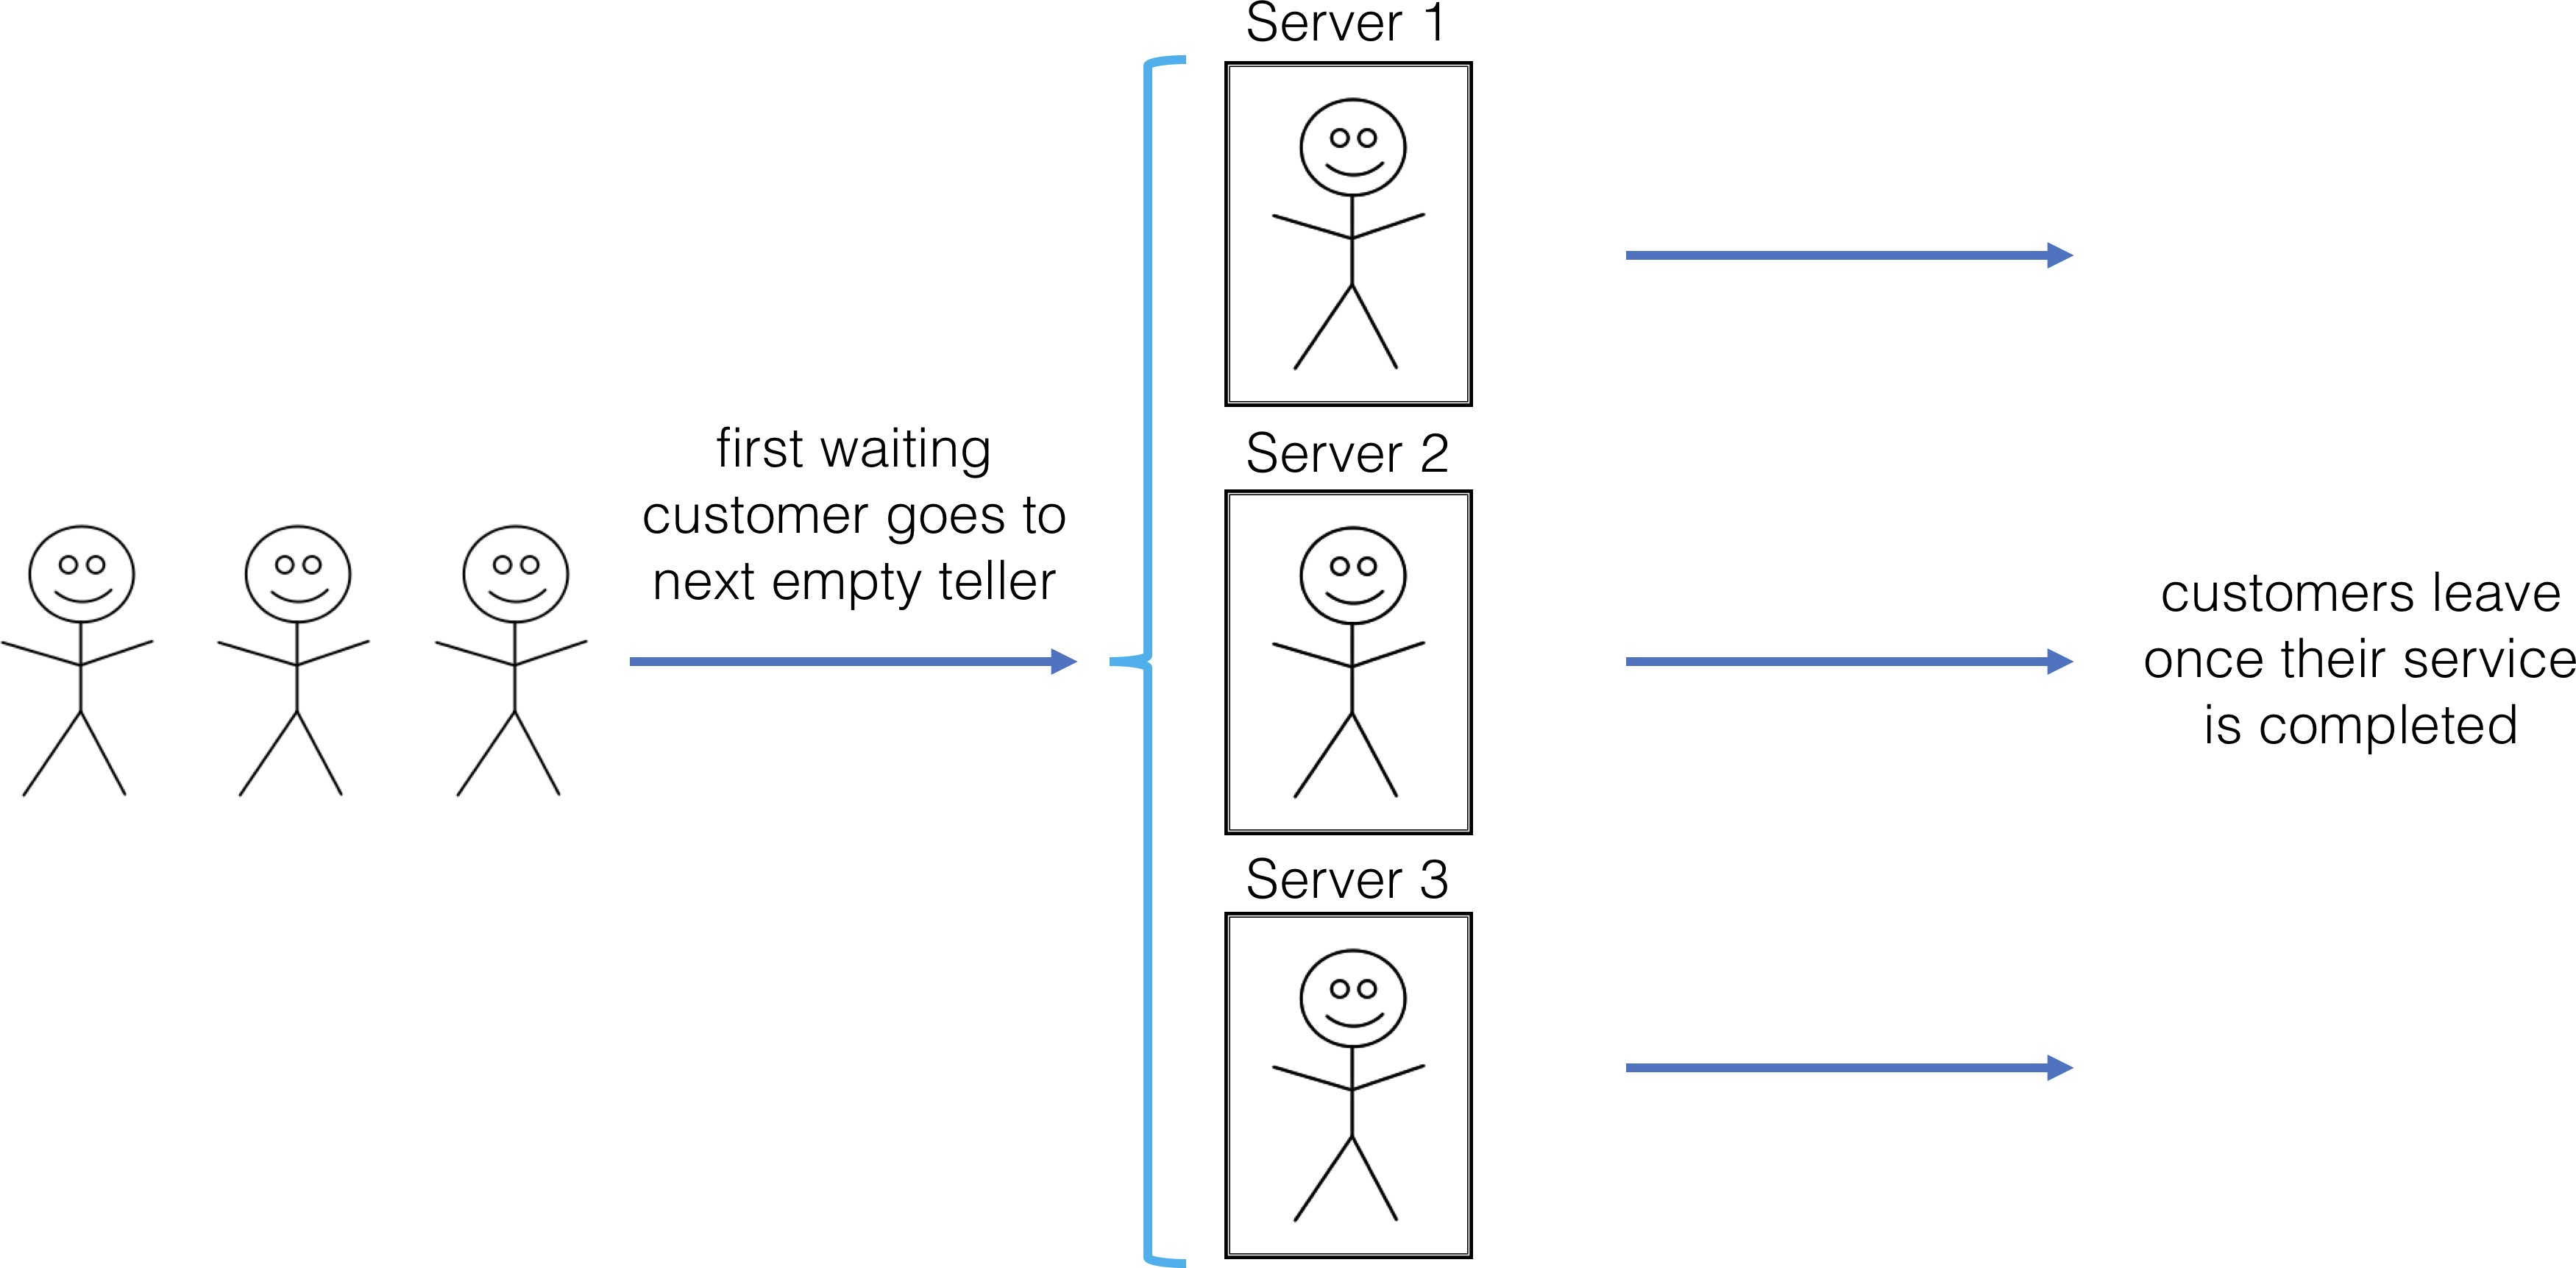
\includegraphics[width=0.49\textwidth]{Images/fig1Queue.png}
	\caption[\small Single line at bank with $3$ tellers]{\small Single line at bank with three tellers -- $M/M/3/\textrm{FCFS}/20/\infty$.}
	\label{fig:1}
\end{figure}
\subsection{Birth-Death Processes}
\begin{figure}[!t]
	\centering
		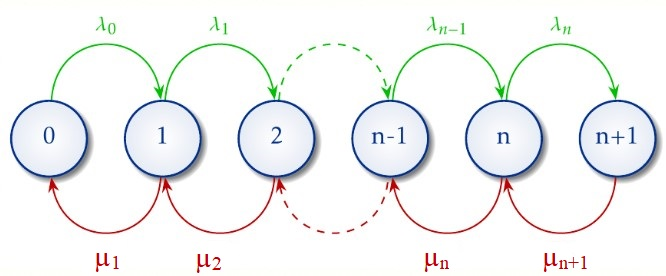
\includegraphics[width=0.49\textwidth]{Images/fig2Queue.jpg}
	\caption[\small Birth-death process]{\small Birth-death process; queueing states indexed by integers; birth rates and death rates indicated by $\lambda_n$ and $\mu_m$, respectively (source unknown).}
	\label{fig:2}\hrule
\end{figure}
The \textbf{state of a queueing system} at time $t$ is defined to be the number of customers in the queuing system, either waiting in line or in service, at time $t$. At $t = 0$, the state of the system is  the initial number of customers in the system. This state is worth recording because it clearly affects the state at future times $t$. \par Knowing this, we define $P_{i,j} (t)$ as the probability that the state at time $t$ is $j$, given that the state at $t = 0$ was $i$. For large $t$, $P_{i,j} (t)$ becomes independent of $i$ and approaches a limit $\pi_{j}$. This limit is known as the \textbf{steady-state} of state~$j$.\newpage\noindent It is generally incredibly difficult to determine the steps of arrivals and services that lead to a steady-state $\pi_j$. Likewise, starting from a small $t$, it is difficult to determine exactly when a system will reach its steady state $\pi_j$, if such a state even exists. \par For simplicity's sake, when a queuing system is studied, we begin by assuming that the steady-state has already been reached.\newl  
A \textbf{birth-death process} is a Markov process in which states are indexed by non-negative integers, and transitions are only permitted between ``neighbouring'' states. After a ``birth'', the state increases from $n$ to $n+1$; after a ``death'', the state decreases from $m$ to $m-1$. Typically, we denote the set of birth rates and death rates by $\lambda_n$ and $\mu_m$, respectively (see Figure~\ref{fig:2}). \textbf{Pure birth} processes are those for which $\mu_m=0$ for all $m$; \textbf{pure death} processes those for which $\lambda_n=0$ for all $n$. The  \textbf{steady-state solution} of a birth-death process, i.e. the probability $\pi_n$ of being in state $n$, \textit{can} actually be computed: 
\begin{align} \pi_{n} &= \pi_{0}\frac{\lambda_{0} \lambda_{1} \cdots \lambda_{n-1}}{\mu_{1} \mu_{2} \cdots \mu_{n}},\quad  \text{for    } n=1,2,\cdots,\label{eq:ssbr}
\end{align}
where $\pi_{0}$ is  the probability of being in state 0. It can further be shown  \cite{QS_K1} that:
$$ \pi_{0} = \frac{1}{1+ \sum^{\infty}_{n=1} \prod^{n-1}_{j=0} \frac{\lambda_{j}}{\mu_{j+1}}}.$$ 

\subsection{Little's Queuing Formula}
It is often the case that clients and end users are interested in determining the amount of time that a typical customer spends in the queuing system. Let $W$ be the \textbf{expected waiting time} spent in the queuing system, including time in line plus time in service, and $W_{q}$ be the \textbf{expected time a customer spends waiting in line}. Both $W$ and $W_{q}$ are computed under the assumption that the steady state has been reached. By using a powerful result known as \textbf{Little's queuing formula}, $W$ and $W_{q}$ are easily related to the number of customers in the queue and those waiting in line. \newl  For any queuing system (or any subset of a queuing system), consider the following quantities:
\begin{itemize}[noitemsep]
\item $\lambda = $  average number of arrivals entering the system per unit time; 
\item $L =$  average number of customers present in the queuing system;
\item $L_{q} = $  average number of customers waiting in line;
\item $L_{s} = $  average number of customers in service;
\item $W = $  average time a customer spends in the system;
\item $W_{q} = $  average time a customer spends in line, and
\item $W_{s} = $  average time a customer spends in service.
\end{itemize}
Customers in the system can only be found in the queue or being serviced, so that $L = L_{q} + L_{s}$ and $W = W_{q} + W_{s}$. In these definitions, all averages are steady-state averages. For most queuing systems in which a steady-state exists, Little's queuing formula can be summarized as 
\begin{align*}
L &=  \lambda W, \quad L_{q} = \lambda W_{q}, \quad\mbox{and}
\quad L_{s}= \lambda W_{s}.
\end{align*}
\begin{Example} If, on average, 46 customers enter a restaurant each hour it is opened, and if they spend, on average, 10 minutes waiting to be served, then we should expect $46\cdot 1/6 \approx 7.7$ customers in the queue at all time (on average).   \end{Example}

